\documentclass[11pt,a4paper]{article}
\usepackage[margin=22mm]{geometry}
\usepackage{amsmath,booktabs,graphicx,siunitx,hyperref}
\title{NAUSICAA: comparison of 10 and 20 ms buckets}
\author{Numerical study}
\date{\today}
\begin{document}
\maketitle
\section{Circuit and input}
The comparison uses the 180 nm CSA with M3 and M4 scaled by four in both
width and length. M3 has $W/L=200/2\,\mu\mathrm{m}$ and gate bias
\SI{0.538477478921}{V}; M4 has $W/L=2.88/1.44\,\mu\mathrm{m}$ and gate bias
\SI{0.556803417206}{V}. The external input capacitance is \SI{1.25}{pF},
the feedback capacitance is \SI{3}{fF}, the supply is \SI{1.8}{V}, and the
temperature is \SI{20}{\celsius}. Intrinsic transistor capacitances are
included by LTspice. The corrected supplied model card uses NOIMOD=2.

Ion collection times are uniform over a bucket of duration $\Delta t$.
Each current is calculated for a positive ion approaching the centre of a
square pad of side \SI{0.5}{mm}, at a constant speed of \SI{3}{m/s}, through
a \SI{5}{mm} gap. The pad belongs to an infinite grounded plane bounding a
uniform dielectric half-space. For the weighting potential, the pad is at
unit potential, the surrounding plane is at zero, and the potential tends
to zero at infinity. The integrated current is
$Q_g=e[1-\phi_w(g)]=0.9984124179e$ per ion.
The mean input per ion is
\[
 i_{\Delta t}(t)=\frac{1}{\Delta t}\int_0^{\Delta t}i_1(t-t_a)\,\mathrm{d}t_a.
\]
The single-ion trajectory and current are unchanged when $\Delta t$ changes.

\section{Measurement and noise}
Voltage readings are centred averages of width $T=\SI{300}{\micro\second}$
at the bucket boundaries. The measured voltage difference is
\[
 D=-[\overline V(\Delta t)-\alpha\overline V(0)],\qquad
 \alpha=\exp(-\Delta t/\tau),\qquad\tau=\SI{0.3}{s}.
\]
The coefficient $\tau$ specifies the discharge correction used in the
measurement. The feedback transistor determines the circuit's discharge.
The transient response gives the gain $g=D/N$ at small input charge.
The input-referred noise is $\mathrm{ENC}=\sigma_D/g$.

The stationary output-noise spectrum comes from the saved LTspice noise
analysis of this same circuit and operating point. Its contribution to $D$
is integrated from \SI{0.1}{Hz} to \SI{1}{MHz}, using
\[
 \sigma_D^2=\int S_V(f)\operatorname{sinc}^2(fT)
 \left[(1-\alpha)^2+4\alpha\sin^2(\pi f\Delta t)\right]\,\mathrm{d}f,
 \qquad\operatorname{sinc}(x)=\frac{\sin(\pi x)}{\pi x}.
\]
Finite-charge transients provide the quoted signal-to-noise ratios and the
integer thresholds. Noise is evaluated about the quiescent operating point.

\section{Results}
\begin{center}
\begin{tabular}{lrr}
\toprule Quantity & 10 ms & 20 ms \\\midrule
Noise of the voltage difference (mV) & 2.556 & 3.042 \\
Calibrated gain ($\mu$V/ion) & 27.020 & 27.127 \\
ENC ($e^-$ RMS) & 94.61 & 112.14 \\
Minimum ion count for $S/N>5$ & 474 & 562 \\
Nominal discharge correction $\alpha$ & 0.967216 & 0.935507 \\
Ideal-gain charge estimate / input charge & 0.5152 & 0.5259 \\
Previous packet residual (\%) & 3.07 & 5.75 \\
Second packet excess, $N=1000$ (\%) & 2.82 & 5.50 \\
$S/N$, 1000 ions & 10.5571 & 8.9067 \\
$S/N$, 2000 ions & 21.0879 & 17.7912 \\
\bottomrule
\end{tabular}
\end{center}
The ideal-gain estimate uses
$\widehat Q=3\,\mathrm{fF}\,[\Delta t/\tau]/(1-\alpha)\,D$.
Its ratio to the input charge describes the finite-gain voltage reduction.
The ENC and the signal-to-noise ratios use the gain calibrated with the
simulated input.

At a fixed arrival rate of 100 ions/ms, the populations are 1000 and 2000
ions. The signal-to-noise ratio increases from 10.56 to 17.79,
a factor 1.685. At the assumed bulk drift speed of \SI{0.1}{m/s},
the longitudinal bucket lengths are 1 and 2 mm.
\begin{center}
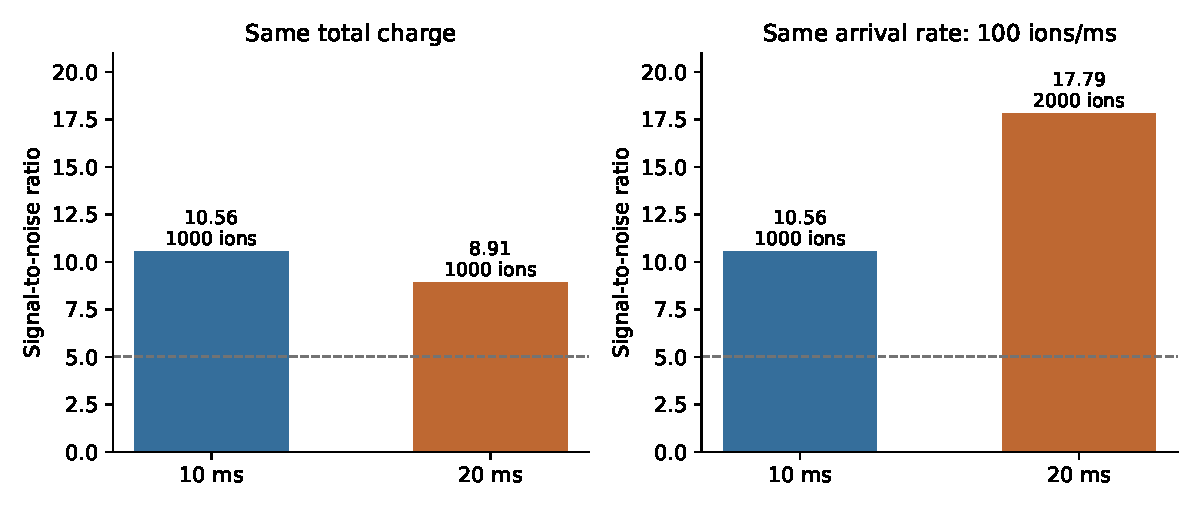
\includegraphics[width=.94\linewidth]{bucket_comparison.pdf}
\end{center}

An isolated packet also produces a residual in the following empty bucket.
The table gives this residual relative to the signal in the packet's own
bucket. For two consecutive packets of 1000 ions each, direct LTspice
transients give the listed excess in the second measurement relative to
an isolated packet. The present correction leaves a larger contribution
from the preceding bucket at 20 ms. A readout calibration must account for
this contribution when reconstructing successive bucket charges.

\section{Numerical checks}
The input PWL waveforms preserve the finite-gap charge. The current is
integrated over each numerical bin before constructing the PWL source.
The maximum timestep and input bin width are both reduced from 5 to
\SI{2.5}{\micro\second}. The largest relative change in a tested finite-charge
signal is \num{1.9e-06}. Noise spectra at 200 and 400 points per decade differ in
filtered RMS noise by less than \num{8e-07}; increasing the quadrature order
from 8 to 16 changes it by less than \num{2.5e-14}.
The new 10 ms gain differs from the saved M3/M4 study by \num{9.7e-06}.

The counts bracketing $S/N=5$ are checked directly:
\begin{center}
\begin{tabular}{rrrrr}
\toprule Bucket & Failing $N$ & $S/N$ & Passing $N$ & $S/N$ \\\midrule
10 ms & 473 & 4.996768 & 474 & 5.007326 \\
20 ms & 561 & 4.999344 & 562 & 5.008250 \\
\bottomrule
\end{tabular}
\end{center}
The convergence errors are less than one tenth of the distance of each
bracketing result from the threshold. Independent tests check the finite-gap
charge by integrating the Ramo weighting field, the scaling of uniform current
with bucket duration, cancellation of an exponential baseline, and the
white-noise limit of the filter.

\section{Reproduction}
Configuration: \texttt{config/bucket\_study.toml}.
Each duration has its own \texttt{10ms/} or \texttt{20ms/} directory under
\texttt{results/ltspice/bucket\_scan/}, containing input currents, LTspice decks,
readable logs, raw HDF5 data and reduced HDF5 results. SHA-256 hashes record
the model, circuit, input, acquisition and reduction code, and noise source.
The earlier studies remain in their original directories.
See the study README for commands. The report and figure are generated by
\texttt{scripts/present\_bucket\_study.py} from the saved reduction.
\end{document}
